\documentclass[notitlepage,a4paper,twoside,10pt]{article}

% \usepackage{mathpazo} 
\usepackage{ngerman} 
\usepackage[latin1]{inputenc} 
\usepackage[T1]{fontenc} 
\usepackage[pdftex]{graphicx} 
\usepackage[pdftex,bookmarks=true,colorlinks,linkcolor=blue,urlcolor=blue,citecolor=blue]{hyperref}

\sloppy

%opening
\title{Zensur im Internet umgehen}
\date{\today}

\hypersetup {
    pdftitle= {Umgehung von Zensur im Internet}
    pdfkeywords= {Zensur DNS-Server}
}


\begin{document}
\maketitle
\tableofcontents

\newpage
\section{Einf�hrung der Zensur in Deutschland}

Die Zensur Neusprech: Access-Blocking) sollte in Deutschland unter dem Deckmantel des Kampfes gegen Kinderpornografie im Internet eingef�hrt werden. Inzwischen hat die Zivilgesellschaft diesen Versuch gestoppt. Trotzdem wird dieser Abschnitt Bestandteil des Privacy-Handbuches bleiben, als Beispiel f�r eine Kampagne und erfolgreichen Widerstand der B�rger.\\

Besonders verkn�pft mit dem Versuch der Einf�hrung einer Internetzensur sind Frau von der Leyen als Familienministerin, Herr Sch�uble als Innenminister und Herr v. Guttenberg. Frau von der Leyen wurde daf�r mit dem Big Brother geehrt. Sie wurde nicht m�de zu behaupten, es g�be einen Millionen Euro schweren Massenmarkt, der durch Sperren von Websites ausgetrocknet werden kann. Ihre Aussagen wurden �berpr�ft und f�r falsch befunden.\\

Die Ermittler vom LKA M�nchen sind der Meinung, dass bei der Verbreitung von Kinderpornographie Geld kaum eine Rolle spielt. Es gibt selten organisierte Strukturen:

\begin{quote}
   \textit{Die �berw�ltigende Mehrzahl der Feststellungen, die wir machen, sind kostenlose Tauschringe, oder Ringe, bei denen man gegen ein relativ geringes Entgelt Mitglied wird, wo also nicht das kommerzielle Gewinnstreben im Vordergrund steht. Von einer Kinderpornoindustrie zu sprechen, w�re insofern f�r die Masse der Feststellungen nicht richtig. (Quelle: S�ddeutsche Zeitung)}
\end{quote}

Ermittler des LKA Niedersachsen best�tigten gegen�ber Journalisten der Zeitschrift ct die Ansicht, dass es keinen Massenmarkt von Websites im Internet gibt. Die sogenannte ``harte Ware'' wird nach ihrer Einsch�tzung �berwiegend per Post versendet. Das Internet (vor allem E-Mail) wird nur genutzt, um Kontakte anzubahnen.\\

Auch die \textit{European Financial Coalition} kommt zu dem Schluss, das es keinen Massenmarkt f�r Kinderpronografie gibt. In den Jahren 2009/2010 ist die Zahl der Angebote im Netz au�erdem deutlich gesunken.\\

Kann es sein, dass diese Erkenntnisse in der Regierung nicht bekannt sind? In der Antwort auf eine parlamentarische Anfrage beweist die Regierung jedenfalls ein hohes Ma� an Unkenntnis zu dem Thema:

\begin{quote}
   Frage: In welchen L�ndern steht Kinderpornographie bislang nicht unter Strafe?\\
   Antwort: \textit{Dazu liegen der Bundesregierung keine gesicherten Kenntnisse im Sinne rechtsvergleichender Studien vor.}\\

   Frage: �ber welche wissenschaftlichen Erkenntnisse verf�gt die Bundesregierung im Zusammenhang mit der Verbreitung von Kinderpornographie.\\
   Antwort: \textit{Die Bundesregierung verf�gt �ber keine eigenen wissenschaftlichen Erkenntnisse...}\\

   Frage: Auf welche Datengrundage st�tzt sich die Bundesregierung bei der Einsch�tzung des kommerziellen Marktes f�r Kinderpornographie in Deutschland?\\
   Antwort: \textit{Die Bundesregierung verf�gt �ber keine detaillierte Einsch�tzung des kommerziellen Marktes f�r Kinderporngraphie...}\\

\end{quote} 
Und basierend auf diesem Nicht-Wissen wird....

\subsubsection*{Die erste Stufe}
Am 17.04.09 unterzeichneten die f�nf Provider Deutsche Telekom, Vodafone/Arcor, Hansenet/Alice, Telefonica/O2 und Kabel Deutschland freiwillig einen geheimen Vertrag mit dem BKA. Dieser Vertrag verpflichtet die Provider, eine Liste von Websites (bzw. Domains) umgehend zu sperren, die das BKA ohne rechtstaatliche Kontrolle zusammenstellt. Statt der gesperrten Website soll ein Stopp-Schild angezeigt werden. Soweit bekannt geworden ist, soll die Sperrung soll durch eine Kompromittierung des DNS-Systems umgesetzt werden.\\

\subsubsection*{Die zweite Stufe}
Am 18.06.09 hat der Deutsche Bundestag ein \textit{Gesetz zur Bek�mpfung der Kinderpornografie in Kommunikationsnetzen} verabschiedet. Das Gesetz ist technikoffen formuliert. Neben den (ungeeigneten) DNS-Sperren sollen auch tiefere Eingriffe in die Kommunikation zul�ssig und angemessen sein. Diskutiert werden IP-Adress-Sperren, kombiniert mit einer Analyse des Datenverkehrs.\\

Das Gesetz zwingt Provider mit mehr als 10.000 Kunden dazu, die im Geheimen vom BKA erstellten Sperrlisten umzusetzen und bei Aufruf einer entsprechenden Website eine Stopp-Seite anzeigen. Die Sperrliste soll durch ein zahnloses Experten-Gemium stichprobenartig mindestens viertelj�rlich �berpr�ft werden. Diese Experten soll der Bundesdatenschutzbeauftragtem berufen.\\

Eine Begrenzung der Sperrma�nahmen auf kinderpornografische Angebote au�erhalb der M�glichkeit der Strafverfolgung ist nicht vorgesehen. Es wurde bereits im Vorfeld die Ausweitung der Internetsperren von verschiedenen Politikern gefordert. Die Aussage von Herrn Bosbach (CDU) ist eigentlich an  Eindeutigkeit nicht zu �berbieten:

\begin{quote}
   \textit{Ich halte es f�r richtig, sich \textbf{erstmal} nur mit dem Thema Kinderpornografie zu befassen, damit die �ffentliche Debatte nicht in eine Schieflage ger�t.}
\end{quote}

Eine konsequente Umsetzung des Subsidarit�tsprinzips \textit{L�schen vor Sperren} ist im Gesetz ebenfalls nicht vorgesehen. Es soll der Einsch�tzung des BKA �berlassen bleiben, ob zu erwarten ist, dass der Provider ein indexiertes Angebot in angemessener Zeit vom Netz nimmt oder eine Internet-Sperre eingerichtet wird. Es besteht keine Verpflichtung f�r das BKA, die Hoster der beanstandeten Websites zu kontaktieren und um L�schung der Angebote zu bitten.

\subsubsection*{Ein Schritt zur�ck}
Im Oktober 2009 hat die Regierungskoalition von CDU und FDP beschlossen, das Gesetz erst einmal nicht umzusetzen. Das BKA soll f�r ein Jahr keine Sperrlisten an die Provider liefern, sondern die Webseiten nach M�glichkeit l�schen lassen. Nach Abauf der Evaluierung soll das Ergebniss gepr�ft und �ber die Einf�hrung von Sperren nochmals beraten werden.\\

Mit einem ``Anwendungserlass'' f�r das BKA hat die Bundesregierung ein vom Deutschen Bundestag beschlossenes Gesetz nicht umgesetzt sondern erst einmal aufgeschoben. Die Ansammlung von Adligen und Mitgliedern der Hochfinanz in unserer Regierung glaubt also, �ber dem Parlament zu stehen. Formal sicher eine seltsame Auffassung von Demokratie.\\

Im April 2011 wurde das Zugangserschwernisgesetz end�ltig beerdigt. Auch die Bef�rworter der Zensur mussten einsehen, dass ein L�schen von Bildmaterial �ber dokumentiertem Missbrauch durch internationale Zusammenarbeit m�glich ist.

\subsubsection*{Umweg �ber die EU}
Nachdem die Zensurma�nahmen in Deutschland nicht durchsetzbar waren, begann eine Kampagne der EU-Kommision. Alle Mitgliedsl�nder sollten zum Aufbau einer Sperrinfrastruktur gegen Kinderpornografie verpflichtet werden. Besonders hervorgetan als Bef�rworterin einer solchen Regelung hat sich Cesilia Malstr�m, die EU-Kommisarin f�r innere Angelegenheiten.\\

\begin{figure}[htb]
\begin{center}

\includegraphics[scale=0.5]{../screenshots/censilia_idee.jpg}
\caption{Quelle: http://i227.photobucket.com/albums/dd41/Scoti17/Malmstrm.jpg}
\label{abb:censilia}
\end{center}
\end{figure}

Das Vorgehen erinnert stark an die Vorratsdatenspeicherung. Der deutsche Bundestag lehnte 2001 die VDS als nicht verfassungskonform ab und kurze Zeit sp�ter kommt eine EU-Richtlinie, die alle Mitgliedsl�nder zur Umsetzung der VDS verpflichten sollte. Das gleiche Spiel beim Zugangserschwernisgesetzt?

\subsubsection*{ACTA, Urheberrecht und Gl�cksspiel}
Parallel zu dieser Entscheidung werden auf internationaler Ebene Abkommen vorbereitet, welche die Einf�hrung einer Zensurinfrastruktur f�r Deutschland verbindlich vorschreiben sollen. In Dokumente zu den ACTA-Geheimverhandlungen wird eine Zensurinfrastruktur zur Verhinderung von Urheberechtsverletzungen gefordert, die internationale Konferenz zum Schutz der Kinder fordert eine Zensurinfrastruktur und auch die Absicherung des staatlichen Gl�ckspiel Monopols soll als Vorwand f�r Sperren im Netz dienen.\\

Wie bei der Einf�hrung der Vorratsdatenspeicherung verfolgen die Verfechter des �berwachungsstaates ihre Ziele hartn�ckig und auf mehreren Wegen.



\subsubsection*{Die Zensur erfolgt auf vielen Ebenen}
Die Einf�hrung der Zensur umfasst nicht nur effektive technische Sperrma�nahmen. Sie wird auch durch juristische Schritte begleitet. Einige Beispiele:
\begin{itemize}
\item Das Forum \textit{Politik global} sollte auf Betreiben des LKA Berlin im Mai 2009 wegen Volksverhetzung geschlossen werden. Das AG Tiergarten in Berlin hat der Klage stattgegeben. Das Urteil des AG Tiergarten ist uns nicht im Wortlaut bekannt. Auf der Website haben wir aber keine Nazi-Propaganda gefunden sondern Israel- und NATO-kritische Themen sowie Hinweise auf Missst�nde in Deutschland und International.\\

Die Domain wurde gel�scht. Da helfen auch keine unzensierten DNS-Server. Die Webseite war f�r einige Zeit weiterhin noch unter der IP-Adresse erreichbar, da der Server nicht in Deutschland stand. Eine neue Doamin wurde registriert, ist derzeit aber auch nicht mehr erreichbar.

\item Am 21. Mai 2009 ver�ffentlichte Spiegel-Online einen Artikel �ber Bestechung von Politikern durch den Telekom Konzern. Dr. Klemens Joos sowie die EUTOP International GmbH wurden in dem Artikel genannt und schickten ihre Anw�lte los, um den Artikel zu entfernen. Sie sahen ihre Rechte in erheblicher Weise beeintr�chtigt. (Der Artikel stand bei Wikileaks weiterhin zum Download zur Verf�gung.)

\item Wikipedia ist immer wieder das Ziel von Zensurbem�hungen. Unliebsame Artikel werden unterdr�ckt oder modifiert. \textit{Man bem�he sich um Neutralit�t}, sagte Gr�nder J. Wales bei der letzten Wikipedia-Konferenz. Aber das ist scheinbar nicht leicht umsetzbar. In der israelischen Wikipeadia fehlt jegliche kritische Bemerkung an der Politik Isreals, wie der Blogger Richard Silverstein kritisch feststellte. Pakistan hat anl�sslich der 2011 Balochistan International Conference Informationen �ber Occupation in der englischen Wikipeadia entfernen lassen und vieles andere mehr. 

\item Das Suchmaschinen ihre Links zensieren ist seit l�ngerem bekannt. Die bei Wikileaks aufgetauchte Sperrliste des ehemaligen Suchdienstes Lycos oder die Sperrlisten von Baidu sind interessant.\\
\end{itemize}

\section{Strafverfolgung von Kinderpornografie}
W�hrend die Einf�hrung von Internet-Sperren f�r die derzeitige Regierung ``ein in vielerlei Hinsicht wichtiges Thema ist'', (v. Guttenberg), scheint die Verfolgung der Anbieter eher niedrige Priorit�t zu genie�en.

\subsubsection*{Wo stehen die Server?}
Im scusiblog \href{https://scusiblog.org}{https://scusiblog.org} findet man Analysen zu verschiedenen europ�ischen Filterlisten. In der L�nderwertung belegt Deutschland stets einen beachtlichen vorderen Platz bei der Ver�ffentlichung von Material mit dokumentiertem Kindesmissbrauch. Eine Zusammenfassung der Sperrlisten der Schweiz, D�namark, Finnland und Schweden (2008) lieferte folgende Zahlen:

\begin{center}
\begin{tabular}{l|c}
Land & Anzahl der Websites\\
\hline
USA & 3947\\
Australien & 423\\
Niederlande & 333\\
\textbf{Deutschland} & \textbf{321}\\
S�d-Korea & 95\\
Kanada & 88
\end{tabular}
\end{center}


Da diese in Deutschland gehosteten illegalen Angebote bei befreundeten Polizeien bekannt sind, stellt sich die Frage, warum sie bisher nicht entfernt und die Betreiber zur Rechenschaft gezogen wurden. Nahezu alle Provider unterst�tzen Ma�nahmen gegen Kinderpornos. Es gen�gt ein Anruf, um das Angebot innerhalb weniger Stunden zu schlie�en. Auch die bei regierungskritischen Themen als \textit{bullet proof} geltenden Hoster wie z.B. MediaOn und noblogs.org kennen bei KiPo kein Pardon.\\

Wenn das BKA kinderpornografische Websites kennt, die auf eine zuk�nftige Sperrliste gesetzt werden sollen, warum werden die Seiten nicht abgeschaltet und die Betreiber zur Verantwortung gezogen? Eine internatione Zusammenarbeit sollte bei diesem Thema kein Problem sein.\\

Zwei Jahre sp�ter war ein Teil der Webangebote noch immer online. Der AK Zensur lie� ganz ohne polizeiliche Vollmacht einige der seit zwei Jahren auf der d�nischen Sperrliste stehenden Webseiten innerhalb von 30min schlie�en. Warum hat ds BKA zwei Jahre lang nichts unternommen?

\subsubsection*{Der lange Dienstweg des BKA}
In einer Studie der Univerit�t Cambridge wurde untersucht, wie lange es dauert, um strafrechtlich relevante Websites zu schlie�en. Phishing-Websites werden innerhalb von 4 Stunden geschlossen. Bei Websites mit dokumentierten Kindesmissbrauch dauert es im Mittel 30 Tage!\\

Frau Krogmann (CDU) antwortete auf eine Frage bei abgeordnetenwatch.de, dass das BKA kinderpornografische Websites nicht schneller schlie�en kann, weil \textbf{der Dienstweg} eingehalten werden muss.\\

Noch mal ganz langsam: 

\begin{enumerate}
   \item Weil das BKA den Dienstweg einhalten muss, k�nnen Websites mit dokumentierten Kindesmissbrauch nicht kurzfristig geschlossen werden?
\item Das mit dem Gesetz zur Einf�hrung von Internet-Sperren rechtsstaatliche Prinzipien verletzt und Grundrechte eingeschr�nkt werden sollen (Grundgesetz Artikel 5 und 10), ist nebens�chlich, wenn auch nur einem Kind damit geholfen werden kann?
\end{enumerate}
Das Gutachten des Wissenschaftlichen Dienstes des Bundestages (WD 3 - 3000 - 211/09) zeigt, dass das BKA auch ohne Zensur wesentlich mehr gegen dokumentierten Kindesmissbrauch tun k�nnte.\\

Wie frustrierend dieser lange Dienstweg und die mangelhafte Unterst�tzung der Strafverfolger sind, zeigt Oberstaatsanwalt Peter Vogt. Die Suedeutsche Zeitung bezeichnet ihn als Pionier der Strafverfolgung von Kinderpornografie. Ab Jan. 2010 steht Herr Vogt f�r diese Aufgabe nicht mehr zur Verf�gung. Er hat wegen unhaltbarer Zust�nde in den Polizeidirektionen das Handtuch geworfen.\\

Interessant ist, dass das BKA eine mit hohen Kosten verbundene Sperr-Infrastruktur aufbauen m�chte, selbst aber nur 6,3 (!) Planstellen f�r die Verfolgung von dokumentiertem Missbrauch bereitstellt. 

\subsubsection*{Die Internet-Sperren sind kontraproduktiv}
Die geplanten Sperren von Websites mit Anzeige einer Stopp-Seite sind f�r die konsequente Verfolgung der Straftaten kontraproduktiv.\\

Mit der Anzeige der Stopp-Seite sollen die Daten des Surfers an das BKA zwecks Einleitung der Strafverfolgung �bermittelt werden. Gleichzeitig wird der Konsument kinderpornografischen Materials jedoch gewarnt und kann alle Spuren beseitigen. Ohne Nachweis der Straftat ist eine rechtsstaatliche Verurteilung jedoch nicht m�glich.\\

\section{Die Medien-Kampagne der Zensursula}
Der Gesetzgebungsprozess wurde von einer breiten Medien-Kampagne begleitet. Die Gegner der Zensur wurden direkt und indirekt als P�dophile oder deren Helfer verunglimpft, es wurde ein Gegensatz von \textit{``Meinungsfreiheit im Internet``} versus \textit{``Schutz der Kinder``} konstruiert und viel mit fragw�rdigem Zahlenmaterial, unwahren Behauptungen und suggestiven Umfragen argumentiert.\\

 Das fragw�rdige Zahlenmaterial f�r die Kampagne wurde �berwiegend von Innocence in Danger geliefert. Diese Organisation unter F�hrung von Julia v. Weiler und Stefanie v.u.z. Guttenberg war auch wegen undurchsichtiger Gesch�ftsgebaren und undokumentierter Verwendung von Spendengeldern in �ffentliche Kritik geraten.\\

 In den Mainstream-Medien wurde die Argumentation der Bef�rworter der Zensur prominent und ohne kritische Nachfrage wiedergegeben:

\begin{quotation}
        \textit{Es macht mich schon sehr betroffen, wenn pauschal der Eindruck entstehen sollte, dass es Menschen gibt, die sich gegen die Sperrung von kinderpornographischen Inhalten str�uben.} (Karl Theodor v.Guttenberg)
       \end{quotation} 
\begin{quotation}
 \textit{Lassen Datensch�tzer und Internet-Freaks sich vor den Karren der H�ndler und Freunde von Kinderpornografie spannen? Diese Frage muss sich nicht nur Franziska Heine stellen.} (Teaser der Zeitschrift ``Emma'')
\end{quotation}
\begin{quotation}
 \textit{Wir k�nnen es doch als Gesellschaft nicht hinnehmen, das - so wie es die Piratenpartei fordert- Jugendliche und Erwachsene ungehindert Zugang zu Kinderpornos im Internet haben k�nnen...} (S. Raabe, SPD)
\end{quotation}

Das Motto der Gegner der Zensur im Internet lautete \textbf{L�schen statt Sperren}. Das stand auch deutlich in der von Franziska Heine initiierten Petition und wurde auf dem Piraten-Parteitag ebenfalls deutlich gesagt.\\

Weitere Beispiele:
\begin{quotation}
 \textit{
Wir vermissen die Unterst�tzung der Internet Community, die uns sagt, wie wir dem wachsenden Problem der Kinderpornografie Herr werden k�nnen. Diese Stimmen sind bisher kaum zu h�ren.} (v.d.Leyen)
\end{quotation}
Heinrich Wefing, der uns schon �fter aufgefallen ist, sinniert in der \textit{Zeit}:
\begin{quotation}
 \textit{Nun k�nnte man die l�rmende Ablehnung jeder staatlichen Regulierung vielleicht sogar als romatische Utopie bel�cheln, wenn die Ideologen der Freiheit gelegentlich mal selbst einen Gedanken darauf verwenden w�rden, wie sich der Missbrauch des Mediums eind�mmen lie�e.}
\end{quotation} 
Die Nerds vom AK Zensur haben nicht nur Hinweise gegeben, sie haben es auch vorgemacht. \textbf{Innerhalb von 12 Stunden wurden 60 kinderpornographische Internet-Angebote gel�scht} (ganz ohne polizeiliche Vollmacht). Was wird noch erwartet. Sollen wir die Dienstanweisung f�r das BKA formulieren? Ein Gutachten des Wissenschaftlichen Dienstes des Bundestages zeigt, dass das BKA diesem Beispiel folgen k�nnte.\\

\begin{quotation}
 \textit{Die bittere Wahrheit ist, dass bisher nur die H�lfte der L�nder Kinderpornographie �chtet.} (v.d.Leyen)
\end{quotation}
Auf der \textit{``Konferenz zum Schutz vor sexueller Gewalt gegen Kinder und Jugendliche mit Fokus auf neue Medien''} behauptet v.d.Leyen:
\begin{quotation}
 \textit{Nur rund 160 Staaten haben �berhaupt eine Gesetzgebung gegen die Vergewaltigung von Kindern, die von den T�tern aufgenommen und �bers Netz verbreitet wird. 95 Nationen h�tten keine solche Gesetze.}
\end{quotation}
Netzpolitik.org hat sich diese Zahlen genauer angesehen. 193 Staaten haben die UN-Konvention zum Schutz der Kinder ratifiziert und in geltendes Recht umgesetzt. Artikel 34 definiert den Schutz vor sexuellem Missbrauch.\\

Von den 95 Nationen, die lt. v.d.Leyen keine Gesetze gegen Missbrauch Minderj�hriger haben sollen, verbieten 71 Pornografie generell. Das schlie�t dokumentiert Missbrauch ein. Weitere befinden sich im B�rgerkrieg oder in einem verfassungsgebenden Prozess nach einem Krieg. Der Rest hat keine nenneswerte Infrastruktur, um Webserver zu betreiben.\\

\begin{quotation}
 \textit{Wer die Stoppseite zu umgehen versucht, macht sich bewusst strafbar, weil er dann aktiv nach Kinderpornografie sucht.} (v.d.Leyen)
\end{quotation}
Moment mal - es war im III. Reich verboten, Feindsender zu h�ren. Einen vergleichbaren Paragraphen sucht man im Strafgesetzbuch vergeblich. Es steht jedem Nutzer frei, vertrauensw�rdige Internet-Server zu nutzen.

\section{L�schen statt Sperren ist funktioniert}
Die Aktionen des AK-Zensur haben gezeigt, dass L�schen statt Sperren m�glich ist. in einer ersten Aktion wurden  innerhalb von 12 Stunden 60 kinderpornografische Internet-Angebote gel�scht, ohne polizeilche Vollmachten. In einer zweiten Aktion wurde die d�nische Sperrliste analysiert. Seit 2 Jahren gesperrte Webseiten konnten innerhalb von 30min gel�scht werden. Das Beispiel zeigt, dass eine Sperrliste auch oft als Alibi dient und eine weitere Strafverfolgung nicht betrieben wird.\\

Der eco Verband konnte im Jahr 2010 von den gemeldeten Webseiten 99,4\% entfernen. Es wurden 256 Websites mit dokumentiertem Missbrauch gemeldet. Davon wurden 448 im Wirkungsbereich von INHOPE umgehend gel�scht. 204 wurden auf ausl�ndischen Server nach kurzem Hinweis vom Provider gel�scht. Bei zwei Meldungen handelte es sich nicht um strafbares Material.
\newpage
\section{Simple Tricks}
Die besten M�glichkeiten zur Umgehung von Zensur sind \textit{Anonymisierungsdienste} mit Anti-Censorship Funktion wie JonDonym oder Tor. Stehen diese Dienste nicht zur Verf�gung, kann man es auch mit den Simple Tricks versuchen. Die \textit{Simple Tricks} wurden bereits an der ``Great Firewall'' in China erprobt und sind teilweise recht erfolgreich. Das einfache Prinzip ist im Bild \ref{abb:simpletrick} dargestellt.\\

\begin{figure}[hbt]
\begin{center}
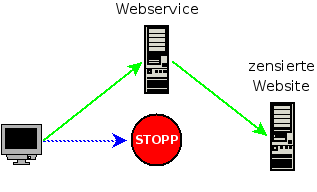
\includegraphics[scale=0.5]{../screenshots/simple_trick.png}
\caption{Prinzip der Simple Tricks}
\label{abb:simpletrick}
\end{center}
\end{figure}

Wenn man auf eine Website nicht zugreifen kann (oder man bef�rchtet, nicht zugreifen zu k�nnen) kann man einen Webdienst im Ausland nutzen. Der Webdienst unterliegt anderen Zensurbedingungen und kann h�ufig auf die gew�nschte Seite zugreifen und �ber den kleinen Umweg unzensiert liefern.\\

\textbf{Hinweis:} Es ist ratsam, Web-Services zu nutzen, die eine \underline{SSL-Verschl�sselung} des Datenverkehrs anbieten. Wer Anonymisierungsdienst wie Tor oder JonDonym nutzen kann, sollte diese M�glichkeit bevorzugen.\\

Einige Vorschl�ge f�r Webdienste:
\begin{enumerate}
   \item \textbf{RSS-Aggregatoren:} sind geeignet, um regelm��ig eine Website zu lesen, die RSS-Feeds anbietet, bspw. Blogs. Man kann sich selbst seine Feeds auf einem Web-Aggregator wie \href{http://www.bloglines.com}{www.bloglines.com} zusammenstellen oder nutzt fertig, themenspezifische Aggregatoren wie z.B. den Palestine Blog Aggregator �ber den Gaza-Krieg.
\item \textbf{SSL-Web-Proxys} bieten ein Formular f�r die Eingabe einer URL. Die Website wird von dem Proxy geholt und an den Surfer geliefert. Dabei werden alle Links der Webseite vom Proxy umgeschrieben, so dass bei einem Klick die folgende Website ebenfalls �ber den Proxy geholt wird. Fl�ssiges Surfen ist m�glich. Um die Filterung des Datenverkehr nach gesperrten W�rtern zu verhindern, sollte man SSL-verschl�sselte Web-Proxys nutzen. Eine Liste von Web-Proxys mit SSL-Verschl�sselung findet man bei Proxy.org oder mamproxy.com oder www.privax.us/. \\

Web-Proxies sind keine Anonymisierungsdienste! Die Admins k�nnten den gesamten Traffic mitlesen, auch bei SSL-verschl�sselten Websites. Sie sind ungeeignet f�r Webangebote, die ein Login mit Passwort erfordern. Viele Web-Proxys speichern die Daten und geben sie auch an Beh�rden weiter, wie der Sahra-Palin-Hack zeigte. Au�erdem k�nnen Webmaster die meisten Web-Proxys austricksen, um Nutzer zu deanonymiseren.
\item \textbf{�bersetzungsdienste:} Man fordert bei einem Web-Translater die �bersetzung einer Website von einer willk�rlichen Sprache (z.B. koreanisch) in die Orginalsprache des Dokumentes an. Der Web-Translater �ndert praktisch nichts. Man kann \href{http://babelfish.yahoo.com}{http://babelfish.yahoo.com} oder \href{http://translate.google.com}{http://translate.google.com} nutzen.
\item \textbf{Low-Bandwidth-Filter:} bereiten Websites f�r Internetzug�nge mit geringer Bandbreite auf. Sie entfernen Werbung, reduzieren die Aufl�sung von Bildern usw. und senden die bearbeitete Website an den Surfen. Man kann sie auch mit High-Speed-DSL nutzen. Steht ein solcher Server im Ausland, hat er h�ufig die M�glichkeit, die gew�nschte Seite zu liefern, z.B. \href{http://loband.org}{http://loband.org}.
\item \textbf{Cache der Suchmaschinen:} Die gro�en Suchmaschinen indexieren Webseiten nicht nur, sie speichern die Seiten auch in einem Cache. Da man Google, Yahoo usw. fast immer erreichen kann: einfach auf den unscheinbaren Link \textit{\underline{cache}} neben dem Suchergebnis klicken.
\item \textbf{E-Mail Dienste:} sind etwas umst�ndlicher nutzbar. Sie stellen die gew�nschte Website per Mail zu. Ein Surfen �ber mehrere Seiten ist damit nat�rlich nicht m�glich. Sie sind aber gut geeignet, unauf�llig einen Blick auf eine gesperrte Website zu werfen. Dem E-Mail Dienst pagegetter.com kann man eine Mail mit der gew�nschten URL der Website im Betreff senden und man erh�lt umgehend eine Antwort-Mail mit der Website. Der Dienst bietet folgende Adresse:
\begin{itemize}
   \item web(�T)pagegetter.com f�r einfache Webseiten.
\item frames(�T)pagegetter.com f�r Webseiten die aus mehreren Framen bestehen.
\item HTML(�T)pagegetter.com liefert die Webseite ohne grafische Elemente aus.
\end{itemize}
\end{enumerate}


\newpage
\section{Unzensierte DNS-Server nutzen}

\includegraphics[scale=0.6]{../grafiken/zensursula_seite_04.png}\\
Am 17.04.09 unterzeichneten diese Provider einen geheimen Vertrag mit dem BKA, in welchem sie sich verpflichtenten, den Zugriff auf eine vom BKA bereitsgestellte Liste von Websites zu sperren. Soweit bekannt wurde, soll die Sperrung haupts�chlich durch Kompromittierung des DNS-Systems erfolgen.\\

\textbf{Hinweis:} Diese leicht zu umgehende Sperre ist im internationalen Vergleich die Ausnahme. Lediglich Australien hat einen vergleichbaren Weg gew�hlt. Die folgenden Hinweise zur Umgehung der Zensur durch Nutzung unzensierter DNS-Server k�nnen nicht auf andere L�nder mit technisch hochger�steter Zensur-Infrastruktur �bertragen werden.\\

Bevor man als Kunde dieser Provider ernsthaft �ber die Nutzung alternativer DNS-Server nachdenkt, sollte man die M�glichkeit eines \textbf{Provider-Wechsels} pr�fen. Das hat folgende Vorteile:
\begin{enumerate}
 \item Man unterst�tzt Provider, die sich gegen die Einschr�nkung der Grundrechte wehren, und �bt Druck auf die Zensur-Provider aus.
 \item Es ist auf f�r IT-Laien eine sichere L�sung, unzensierte DNS-Server zu nutzen, da m�glicherweise Zensur-Provider den Datenverkehr auf eigene, zensierte DNS-Server umlenken, ohne dass man es als Nutzer bemerkt. So leitet Vodafone bspw. bereits seit Juli 09 im UMTS-Netz DNS-Anfragen auf die eigenen Server um. Im DFN Forschungsnetz soll die Nutzung unzensierter DNS-Server durch Sperrung des Port 53 unterbunden werden.
\end{enumerate}

Die deutschen Provider Manitu (\href{http://www.manitu.de}{http://www.manitu.de}) und SNAFU (\href{http://www.snafu.de}{http://www.snafu.de}) lehnten die Sperren ab und werden sie auch nicht umsetzen. SNAFU bietet seinen Kunden an, via Webinterface alternative, unzensierte DNS-Server f�r den eigenen Account zu konfigurieren. Damit entfallen die im folgenden beschrieben Spielereien am privaten Rechner und man hat mit Sicherheit einen unzensierten Zugang zum Web.

\subsubsection*{Was ist ein DNS-Server}
\begin{enumerate}
 \item Der Surfer gibt den Namen einer Website in der Adressleiste des Browsers ein. (z.B. \textit{https://www.awxcnx.de})
\item Daraufhin fragt der Browser bei einem DNS-Server nach der IP-Adresse des Webservers, der die gew�nschte Seite liefern kann.
\item Der DNS-Server sendet eine Antwort, wenn er einen passenden Eintrag findet. (z.B. \textit{62.75.219.7}) oder NIXDOMAIN, wenn man sich vertippt hat.
\item Dann sendet der Browser seine Anfrage an den entsprechenden Webserver und erh�lt als Antwort die gew�nschte Website.
\end{enumerate}
Ein kompromittierter DNS-Server sendet bei Anfrage nach einer indexierten Website nicht die korrekte IP-Adresse des Webservers an den Browser, sondern eine manipulierte IP-Adresse, welche den Surfer zu einer Stop-Seite f�hren soll.\\

Die Anzeige der Stop-Seite bietet die M�glichkeit, die IP-Adresse des Surfers zusammen mit der gew�nschten, aber nicht angezeigten Webseite zu loggen. Mit den Daten der Vorratsdatenspeicherung k�nnte diese Information personalisiert werden.\\

(Diese Darstellung ist sehr vereinfacht, sie soll nur das Prinzip zeigen. Praktische Versuche, das DNS-System zu manipulieren, haben meist zu komplexen Problemen gef�hrt.)

\subsubsection*{Nicht-kompromittierte DNS-Server}

Statt der kompromittierten DNS-Server der Provider kann man sehr einfach unzensierte Server nutzen.  Einige DNS-Server k�nnen auch auf Port 110 (TCP-Porotoll) angefragt werden, falls einige Provider den DNS-Traffic auf Port 53 zum eigenen Server umleiten oder behindern. Wir gehen bei der Konfiguration f�r Windows und Linus darauf n�her ein.\\

Die Swiss Privacy Foundation stellt folgende unzensierten DNS-Server mit aktiviertem DNSSEC zur Verf�gung:
\begin{verbatim}
   87.118.85.241     (DNS-Ports: 53, 110)
   77.109.138.45     (DNS-Ports: 53, 110)
   77.109.139.29     (DNS-Ports: 53, 110)
\end{verbatim}

Der FoeBud bietet einen unzensierten DNS-Server:
\begin{verbatim}
   85.214.20.141
\end{verbatim}

Und der CCC hat nat�rlich auch einen Unzensierten, aber ohne DNSSEC:
\begin{verbatim}
   213.73.91.35
\end{verbatim}


\subsection{WINDOWS konfigurieren}
Wir bezweifeln, das es zur Umgehung der Zensur ausreicht, einfach einen unzensierten DNS-Server zu nutzen. Das am 18.06.09 verabschiedete Gesetz zur Einf�hrung der Zensur ist ausdr�cklich technik-offen formuliert. Es sieht vor, dass die DSL-Provider alle n�tigen Ma�nahmen ergreifen. um den Zugriff auf indexierte Webseiten effektiv zu sperren. Die Nutzung unzensierter DNS-Server kann relativ einfach unterbunden werden. Vodafon leitet im UMTS-Netz bereits alle Anfragen auf eigene DNS-Server um, die Pl�ne des DFN Forschungsnetzes sehen eine Sperrung von Port 53 vor.\\

 Eine M�glichkeit bietet die Verwendung eines nicht �blichen TCP-Ports f�r DNS-Anfragen. Die DNS-Server der GPF k�nnen neben dem �blichen Port 53 auch auf Port 110 angefragt werden. Da WINDOWS die Konfiguration vom Standard abweichender Einstellungen nicht erm�glicht, ist etwas mehr Aufwand n�tig, als die bekannten 27sec.

\subsubsection*{bind9 installieren}
Der Nameserver \textit{bind9} steht auch f�r WINDOWS beim ISC unter der Adresse \href{https://www.isc.org/download/software/current}{https://www.isc.org/download/software/current} zum Download bereit. Nach dem Entpacken des ZIP-Archives ruft man \textit{BINDInstall.exe} als Administrator auf. Als Target-Directory f�r die Installation w�hlt man am besten \textit{C:/bind} und nicht die Voreinstellung.\\

Nach der Installation sind auf der Kommandozeile noch ein paar Nacharbeiten als Administrator n�tig:
\begin{verbatim}
 c:
 cd \bind\bin
 rndc-confgen -a
 mkdir c:\bind\zone
 mkdir c:\bind\log
 cacls c:\bind /T /E /C /G named:F
\end{verbatim} 

Im Verzeichnis \textit{C:/bind/zone} m�ssen die drei Dateien angelegt werden:
\begin{enumerate}
 \item localhost.zone
\begin{verbatim}
 $TTL 86400
 @ IN SOA @ root ( 1 ; serial
 3H ; refresh
 15M ; retry
 1W ; expiry
 1D ) ; minimum
 
 IN NS @
 IN A 127.0.0.1
 IN AAAA ::1
\end{verbatim} 

\item localhost.rev
\begin{verbatim}
 $TTL 86400
 @ IN SOA localhost. root.localhost. ( 1 ; Serial
 3H ; Refresh
 15M ; Retry
 1W ; Expire
 1D ) ; Minimum
 
 IN NS localhost.
 1 IN PTR localhost.
\end{verbatim} 

\item Die Datei \textit{db.cache} l�dt man von \href{ftp://ftp.internic.net/domain/db.cache}{ftp://ftp.internic.net/domain/db.cache} und speichert sie in dem Verzeichnis \textit{C:/bind/zone}. Diese Datei enth�lt die Informationen zu den DNS-Root-Servern.
\end{enumerate}

Abschlie�end konfiguriert man in der Datei \textit{named.conf} in der Sektion \textit{options} die f�r die Weiterleitung genutzten DNS-Server als \textit{forwarders}, welche auch auf Port 110 angefragt werden k�nnen, ein Beispiel:

\begin{verbatim}
options {
    directory "C:\bind\zone";
    allow-query { localhost; };
    max-cache-size 16M;
    cleaning-interval 60;
    listen-on { 127.0.0.1; }; 
 
    forwarders {
       87.118.100.175 port 110;
       94.75.228.29 port 110;
    };  
};
\end{verbatim} 

Wenn die Konfiguration fertig ist, kann man den Dienst mit dem Befehl \textit{net start named} auf der Kommandozeile starten oder �ber die Taskleiste unter \textit{Start - Systemsteuerung - Verwaltung - Dienste} hochfahren.

\subsubsection*{Einstellungen der Internetverbindungen anpassen}
In den Einstellungen der Internetverbindungen wird der lokale bind9 als DNS-Server konfiguriert. In der \textit{Systemsteuerung} ist die Liste der Netzwerkverbindungen zu �ffnen. Ein Klick mit der rechten Maustaste �ffnet das Kontext-Men�, wo man den Eintrag Eigenschaften w�hlt. Der in Bild \ref{abb:dns1} gezeigte Dialog �ffnet sich.\\

\begin{figure}[htb]
\begin{center}
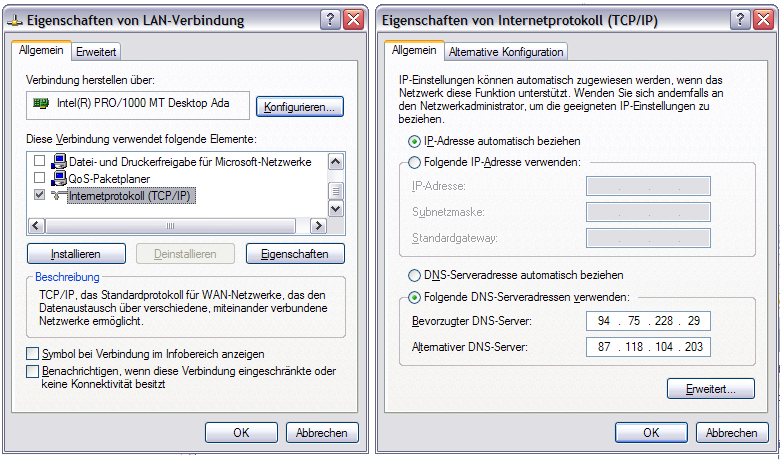
\includegraphics[scale=0.5]{../screenshots/dns_win3.png}
\caption{Konfiguration der DNS-Server (WINDOWS)}
\label{abb:dns1}
\end{center}
\end{figure}

Hier w�hlt man die \textit{TCP-Verbindung} und klickt auf \textit{Eigenschaften}. In dem folgenden Dialog kann man eigene DNS-Server konfigurieren. In dem folgenden Dialog kann man den lokalen bind9 als DNS-Server konfigurieren, indem man als \textit{Bevorzugten DNS-Server} die Adresse \textit{127.0.0.1} eingibt.

\subsection{Linux konfigurieren}
Unter Linux sind nichts-standardm��ige Einstellungen leichter realiserbar. Es ist auch relativ einfach, einen lokalen DNS-Cache zu nutzen, um die zensurfreien DNS-Server nicht �berm��ig zu belasten.\\

\subsubsection*{pdnsd und resolvconf verwenden}
Der \textit{pdnsd} ist ein leichtgewichtiger DNS-Cache-Daemon. Er steht auf allen Linux-Distributionen zur Verf�gung. Unter Debian und Unbuntu installiert man ihn zusammen mit \textit{resolvconf}: 
\begin{verbatim}
 > sudo aptitude install resolvconf pdnsd 
\end{verbatim} 
Bei der Installation des \textit{pdnsd} wird man gefragt, wie die Namensaufl�sung erfolgen soll. W�hlen Sie zuerst einmal \textit{recursive}. Laden Sie die vorbereitete Konfigurationsdatei \href{https://www.awxcnx.de/download/pdnsd-gpfserver.conf}{https://www.awxcnx.de/download/pdnsd-gpfserver.conf} herunter und speichern Sie die Datei im Verzeichnis \textit{/usr/share/pdnsd}.\\ 

Anschlie�end in der Datei /etc/default/pdnsd den AUTO\_MODE anpassen:  
\begin{verbatim}
 START_DAEMON=yes
 AUTO_MODE=gpfserver
 OPTIONS=
\end{verbatim} 
Den Eigent�mer der Config-Datei auf \textit{root} setzen und den Daemon neu starten: 
\begin{verbatim}
 sudo chown root:root /usr/share/pdnsd/pdnsd-gpfserver.conf
 sudo invoke-rc.d pdnsd restart 
\end{verbatim} 
Der DNS-Traffic geht via TCP-Protokoll auf Port 110 zu den unzensierten DNS-Servern. Es ist schwer zu erkennen, dass es sich DNS-Traffic handelt und eine Umleitung auf DNS-Server der Provider ist wenig wahrscheinlich. Zur Sicherheit gelegentlich testen.

\subsubsection*{bind9 und resolvconf verwenden}
Die Pakete \textit{bind9} und \textit{resolvconf} sind in allen Distributionen fertig konfiguriert vorhanden und bieten einen vollst�ndigen DNS-Nameserver. Nach der Installation mit der Paketverwaltung l�uft der Nameserver und ist unter der Adresse 127.0.0.1 erreichbar. Die Tools aus dem Paket \textit{resolvconf} sorgen f�r die automatische Umkonfiguration, wenn \textit{bind9} gestartet und gestoppt wird. F�r Debian und Ubuntu k�nnen die Pakete mit \textit{aptitude} installiert werden:
\begin{verbatim}
 > sudo aptitude install resolvconf bind9
\end{verbatim} 
Die unzensierten DNS-Server sind in der Datei \textit{/etc/bind/named.conf.opions} einzutragen. Die Datei enth�lt bereits ein Muster. Dabei kann optional auch ein nicht �blicher Port angegeben werden:
\begin{verbatim}
 forwarders {
      94.75.228.29 port 110; 
      62.75.219.7  port 110;
 };
 listen-on { 127.0.0.1; };
\end{verbatim} 
(Standardm��ig lauscht der Daemon an allen Schnittstellen, auch an externen. Die Option \textit{listen-on} reduziert das auf den lokalen Rechner.)\\

Wer etwas ratlos ist, mit welchem Editor man eine Konfigurationsdatei anpasst, k�nnte \textit{``kdesu kwrite /etc/bind/named.conf.opions''} oder \textit{``gksu gedit /etc/bind/named.conf.opions''} probieren.\\

Nach der Anpassung der Konfiguration ist \textit{bind9} mitzuteilen, dass er die Konfigurationsdateien neu laden soll:
\begin{verbatim}
   > sudo invoke-rc.d bind9 reload
\end{verbatim} 

\input{../latex/surfen_dns_test}


\end{document}